\section{ISO14443}

\begin{frame}
    \frametitle{ISO14443a e NFC}
    \textbf{Cos'è NFC}\\
    Tecnologia di comunicazione contactless (short range wireless)
    che permette la produzione di dispositivi a basso costo\cite{coskun2013survey}

    \pause

    \textbf{Come funziona}
    \begin{itemize}
        \item<1-> Semplificando il tutto, la comunicazione NFC è equivalente a un trasformatore.
        \item<2-> La trasmissione dell'informazione avviene mediante ASK e Load Modulation\cite{instruments2014iso}
    \end{itemize}
\end{frame}
\note{
    La codifica dell'informazione avviene con una variante di  Manchester Encoding\cite{instruments2014iso}
    
    Uno dei principali vantaggi della tecnologia è che il tag può essere completamente passivo e alimentarsi grazie al campo magnetico generato dal lettore che causa induzione magnetica nella bobina del dispositivo.
}

\begin{frame}
    \begin{figure}
        \centering
        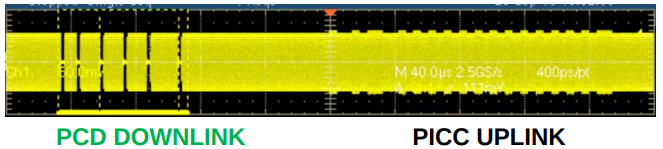
\includegraphics[width=0.85\textwidth]{ISO14443a_COM.png}
        \caption{Traccia della comunicazione tra dispositivo e lettore~\cite{instruments2014iso}}
        \label{fig:iso14443a-trace}
    \end{figure}
    Si noti come la frequenza della portante sia notevolmente elevata\pause

    Ciò permette di avere dei dispositivi (TAG) completamente passivi alimentati dalla portante stessa.
\end{frame}
\note{
    Dall'immagine è possibile osservare come la trasmissione in downlink sia 100\% ASK, dove le tempistiche di bit
    sono notevolmente inferiori ai 13.56MHz della portante.
    Ciò permette al dispositivo di essere completamente passivo e di auto alimentarsi tramite l'effetto trasformatore
    causato dal coupling elettoromagnetico delle due induttanze.
    La trasmissione inversa, dal tag al lettore, di conseguenza non può avvenire allo stesso modo, essendo il tag non in grado di generare
    una portante.
    
    La soluzione è di variare l'impedenza collegata alla spira di ricezione nel tag in modo da utilizzare più corrente.
    Questo genererà una maggiore corrente nel lato trasmettitore che, mediante la resistenza interna di quest'ultimo, causerà una caduta
    di tensione leggibile e interpretabile.
}

\subsection{UUID e anticollisione}
\begin{frame}
    \frametitle{UUID e identificazione multipla di TAG}
    \begin{itemize}
        \item<1-> L'UUID è un codice di univoco che permette l'identificazione dei tag.
        Un generico tag ISO14443-compliant possiede un UUID di 10byte, ma varie implementazioni permettono di avere una lunghezza a partire da 4byte.\cite{nxpmifareuidhandling}
        \item<2-> Mediante il ciclo di identificazione e anticollisione è possibile ottenere la lista di tutti i tag presenti nelle vicinanze del lettore.
        \item<3-> Sarà poi possibile inviare comandi specifici a un solo tag mediante il processo di selezione
    \end{itemize}
\end{frame}
\note{
    Secondo lo standard, durante il processo di discover (Denominato ``anticollision loop'') è possibile dostinguere i tag grazie ai loro ID.

    È interessante notare, leggendo~\cite{nxpmifareev1datasheet}, che sono possibili più iterazioni del ciclo di anticollisione (CL1, CL2, CL3) dove ogni esecuzione incrementa il numero di byte che definiscono l'UUID.

    Risulta quindi che per una carta implementante tutti e tre i livelli di anticollisione l'UUID sarà \textbf{univoco} e lungo 80 bit; mentre per le carte con soli due livelli l'UUID sarà di 56 bit ma pur sempre \textbf{univoco}.
    L'unica implementazione in cui \textbf{non è garantito che il valore sia univoco} è quella base da 32 bit.

    Il protocollo poi prosegue con un paradigma ``select and operate'',
    dove una sessione di comunicazione viene iniziata tramite l'UUID inviato dal lettore. A questo punto tutti i tag nella zona attiva rimarranno in stato IDLE ad eccezione del tag che è stato interpellato.
}

\subsection{Tag MIFARE Classic}
\subsubsection{Struttura della memoria}
\begin{frame}
    \frametitle{MIFARE Classic: Struttura della memoria}
    I tag MIFARE Classic sono tra i più \textbf{semplici} ed \textbf{economici}:
    
    Il tag consiste in un piccolo frontend radio e logico che possa gestire la comunicazione
    e in una memoria non volatile dove salvare le configurazioni.\cite{nxpmifareev1datasheet}

    \begin{figure}
        \centering
        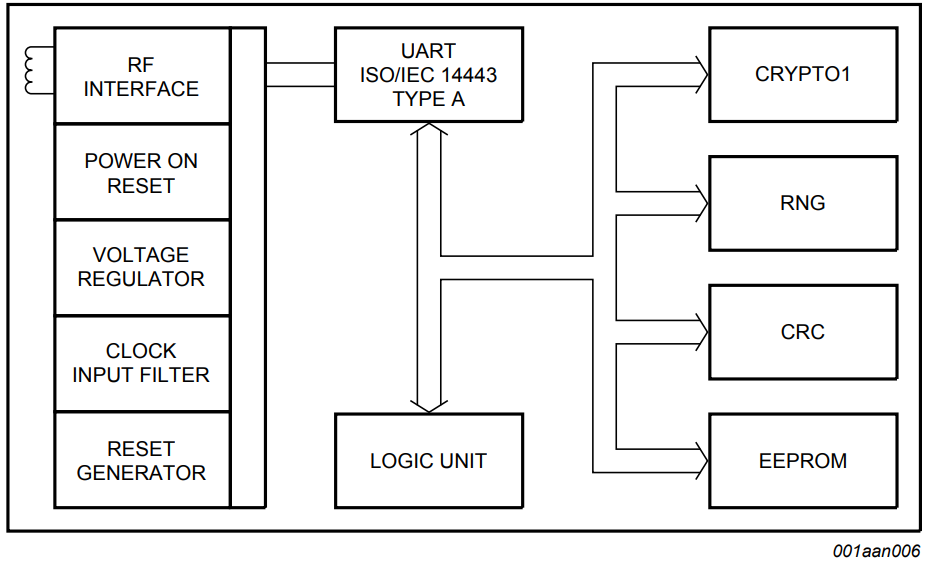
\includegraphics[width=0.3\textwidth]{MIFARE-EV1-INTERNAL_STRUCTURE.png}\cite{nxpmifareev1datasheet}
        \caption{Diagramma dei componenti interni a un chip MIFARE Classic}
        \label{fig:internal-mifare-block-diagram}
    \end{figure}
\end{frame}
\note{
    \footnotesize
    \begin{columns}
        \begin{column}{0.5\textwidth}
            La struttura di un tag MIFARE CLASSIC è da ritenersi interessante.
    
            Dato il ridotto costo del dispositivo ne consegue una bassa complessità elettronica.
            Infatti esso è costituito per una buona parte da componenti standard atti alla gestione della comunicazione e del chip in sè: L'interfaccia radio e il regolatore di tensione infatti sono gli unici componenti analogici presenti sul silicio.

            Successivamente si ha l'unità logica che ha il compito di gestirà la comunicazione e vigilare sulle operazioni, ma quest'ultima non ha grande complessità. L'algoritmo utilizzato è di fatto molto contenuto ed è equivalente a una macchina a stati.

            È interessante notare come la gestione della memoria, in seguito descritta, sia ottimizzata al fine di ridurre i costi.
        \end{column}
        \begin{column}{0.5\textwidth}
            \begin{figure}
                \centering
                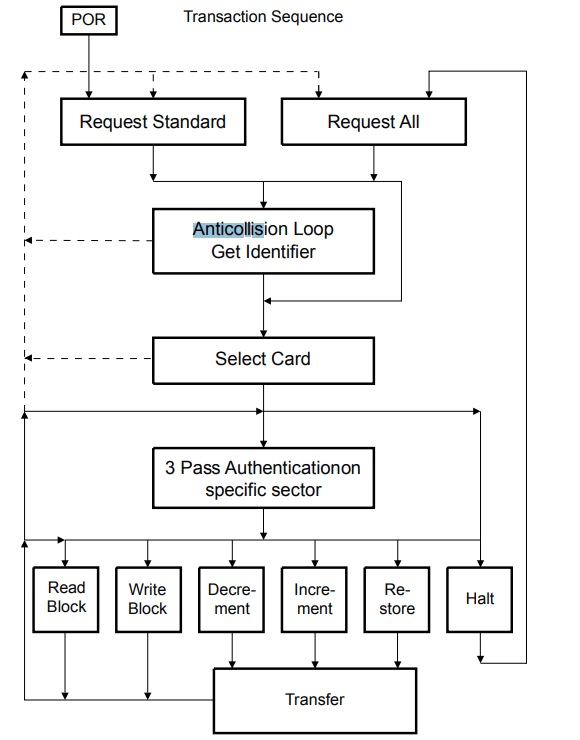
\includegraphics[width=.6\textwidth]{algo_mifare.png}
                \caption{Schema a blocchi della gestione logica di una transazione}
            \end{figure}
        \end{column}
    \end{columns}
}

\begin{frame}
    La memoria è divisa in \textbf{settori} e \textbf{blocchi}:
    \begin{itemize}
        \item <1-> 16 settori \texttt{[0-15]}
        \item <2-> 4 blocchi per settore \texttt{[0-3]}
        \item <2-> Solo tre blocchi per settore possono includere dati \texttt{[0-2]}
        \item <3-> Il blocco \texttt{0:0} è leggibile senza autenticazione, protetto in scrittura e contiene l'UUID e dati del produttore
        \item <4-> I blocchi \texttt{x:3} contengono le chiavi di scrittura e lettura (\textit{KeyA} e \textit{KeyB}), oltre che gli indicatori di protezione (access bits)
    \end{itemize}
\end{frame}
\note{
    È molto interessante notare come, al fine di mantenere bassi i costi di fabbricazione, le memorie sono le responsabili dei i costi (e lo spazio su silicio) più elevati.

    Di conseguenza all'interno dei tag la memoria stessa viene utilizzata per il salvataggio delle chiavi di accesso e delle condizioni.

    È inoltre interessante notare come esistano due diverse chiavi di cifratura per ogni settore: questo è fatto al fine di permettere l'utilizzo diversificato del tag a fronte di un segreto condiviso diverso. Molte volte la chiave A è utilizzata per permettere la sola lettura dei blocchi (escluso quello contenente la chiave B), mentre la chiave B è una chiave master in grado di riprogrammare il tag.

    Bisogna però citare \cite{Courtois2009TheDS}, dove l'autore sottolinea come l'implementazione dell'algoritmo sia una ``waste of silicon'' data la caratteristica dell'offuscamento, dove funzioni identità sono implementate in modi diversi sul die. Questo, moltiplicato per il numero di tag prodotti causa un vero e proprio spreco di materiale.
}

\subsubsection{Lettura e scrittura}
\begin{frame}
    \frametitle{MIFARE Classic: Lettura e scrittura}
    Prima di effettuare qualunque azione sulla memoria è necessario autenticarsi con la chiave adatta al settore in questione.\pause

    Il processo di autenticazione è chiamato \textit{``Three pass authentication sequence''}\cite{nxpmifareev1datasheet}
    e sfrutta un cifrario a flusso
\end{frame}
\note{
    Durante questa procedura il cifrario viene inizializzato in uno stato comune al fine di permettere una trasmissione riservata.
    Lo stato condiviso sfrutta la presenza di nonce casuali per assicurare l'unicità della comunicazione in modo da impedire correlazioni e attacchi replica.
}

\subsubsection{Three pass authentication sequence}
\begin{frame}
    \frametitle{Three pass authentication sequence\cite{garcia2008dismantling}}
    {
        \small
        \begin{columns}[onlytextwidth,T]
            \column{\dimexpr\textwidth-40mm-2mm}
                \begin{itemize}
                    \item <1-> Il tag entra nel campo magnetico del lettore e si accende
                    \item <2-> Protocollo di anticollisione (\textit{Non descritto}) e invio dell'UUID
                    \item <3-> Il lettore effettua una richiesta di autenticazione al blocco richiesto
                    \item <4-> Il tag ritorna un nonce \(n_t\) e lo trasmette in chiaro
                    \item <5-> Il lettore quindi invia il proprio nonce \(n_r\) e la risposta alla challenge \(a_r\)
                            cifrandoli mediante xoring con lo stream proveniente dal cifrario a flusso \(ks_1\) e \(ks_2\)
                    \item <6-> L'autenticazione si conclude con il tag che risponderà alla challenge del reader con \(a_t\) cifrato tramite \(ks_3\)
                \end{itemize}
            \column{40mm}
                \begin{figure}
                    \centering
                    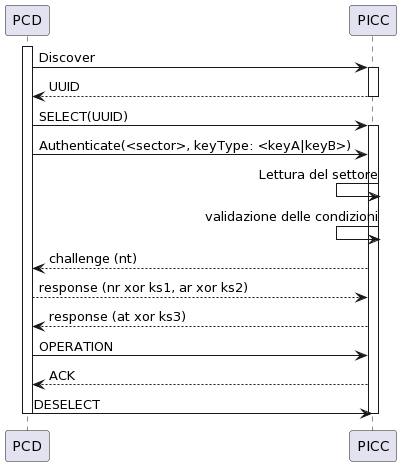
\includegraphics[width=40mm]{AuthSequence.png}
                    \caption{\scriptsize Diagramma di sequenza del processo di autenticazione a un blocco}
                    \label{fig:seq-three-pass-auth}
                \end{figure}
        \end{columns}
    }
\end{frame}
\note{
    Come è possibile vedere dallo schema, il processo di autenticazione inizia con il tag che invia un proprio nonce $n_t$ al lettore, in modo da - idealmente - impedire il riutilizzo di uno stato interno.
    Infatti il nonce è utilizzato in concomitanza con l'UUID e la chiave del settore per inizializzare il cifrario.

    Infatti senza UUID e senza nonce, due tag con chiave uguale potrebbero essere scoperti solamente ascoltando (eavesdropping) le comunicazioni.
    Inserendo l'UUID nell'algoritmo ciò diviene impossibile perchè i tag avranno uno stato diverso in funzione dell'UUID, il quale è unico (o comunque è improbabile che due tag abbiano lo stesso uuid)
    Ciò non ferma però eventuali attacchi che fanno leva sulla ripetizione degli stati iniziali del tag.

    A tal fine viene introdotto il numero casuale deciso dal tag: la sua trasmissione in chiaro non è direttamente un vettore di attacco, ma si vedrà che è stato il metodo utilizzato per scoprire svariate vulnerabilità sull'rng.
}

\begin{frame}[allowframebreaks]
    \frametitle{Three pass authentication sequence\cite{garcia2008dismantling}}
    La scelta dei nonce avviene come dalla seguente illustrazione, dove \(key\) è la chiave condivisa
    (ovvero la chiave che il lettore usa per autenticarsi)
    
    Generazione del tag nonce
    \[n_t = nextRandom()\]
    \[send(n_t)\]

    Dopo l'invio, sia il tag che il lettore inizializzano il proprio cifrario a flusso e computano i primi 32bit del \textit{keystream}
    \[ks_1 = cipherInit(key, uid, n_t)\]

    Generazione del reader nonce
    \[n_r = nextRandom()\]

    Invio del reader nonce (cifrato) e della risposta alla challenge così computata
    \[a_t = suc^2(n_t)\]
    \[ks_2 = cipher(n_r)\]
    \[send(n_r \oplus ks_1); send(a_t \oplus ks_2)\]
    
    Risposta finale
    \[send(suc^3(n_t) \oplus ks_3)\]

\end{frame}
\note{
    Sia la funzione \(suc(v)\) la successiva iterazione del rng con seed \(v\) 
    
    Il processo di scambio di chiavi viene così descritto:~\cite{nxpmifareev1datasheet}
    \begin{itemize}
        \item il tag sceglie il proprio nonce $n_t$ e lo invia al lettore
        \item entrambe le parti inizializzano il proprio cifrario con una funzione della chiave \(key\), \(n_t\) e l'UUID del tag
        \item una volta ottenuto il nonce, il lettore computa i primi 32 bit del keystream, inserendo nel LFSR i 32 bit di una funzione $f(n_t, uuid)$
        \item il lettore genera \(n_r\) e lo invia al tag cifrandolo con \(ks_1\) (\(n_r \oplus ks_1\)); insieme invia la risposta alla challenge \(a_r = suc^2(n_t)\), seconda iterazione del RNG con seed $n_t$, cifrata con i secondi 32 bit ottenuti aggiornando il proprio cifrario con $n_r$
        \item il tag, quindi, aggiorna il proprio cifrario con \(n_r\) e verifica che $a_r$ sia valida.
        \item per completare l'autenticazione viene quindi inviato \(suc^3(n_t)\) cifrato con \(k_3\) in modo che Il lettore possa validare il tag.
    \end{itemize}
}

